% Provenance (never printed): see sources/outline_sources.md (Year 3:
% dislocation and diffusion creep; flow laws; deformation maps; shear zones and
% kinematic indicators). Brief: sources/book5/BRIEFS.md, ch. 7. Curves from
% figdata/bachelor-3/flow_laws.py. Exercise and problem values in the Book 5
% scratch calculator calc/ch07.py.
\chapter{变形机制与剪切带}\label{ch:b3:deformation-mechanisms}

在地表，山体中的花岗岩沿断层破碎。在地下二十
千米深处，同一种花岗岩在一条
宽仅数百米的\omterm{def:b3:deformation-mechanisms:shear-zone}{剪切带}中像软糖一样流动，其长石被揉成“眼球”状，石英被拉出
成条带。晶体能不破裂地流动，是因为它从来不完美：
它依靠缺陷运动，每次移动一排原子，或让原子从
晶粒的一个面扩散到另一个面。本章沿着这些机制，从晶格
讲到地球动力学所用的定律，再到说明何种机制占优的\omterm{def:b3:deformation-mechanisms:deformation-map}{变形机制图}，
最后讲\omterm{def:b3:deformation-mechanisms:shear-zone}{剪切带}，岩石正是在其中记录下自己的运动方式。

\begin{recall}
点缺陷、阿伦尼乌斯定律和活化能见
化学各册的大学分册；扩散系数见物理
各册。应力与应变、应变椭圆、简单剪切及其椭圆
（$S_{1,2} = \sqrt{1 + \gamma^2/4} \pm \gamma/2$，长轴与
剪切方向的夹角为 $\theta'$，且 $\tan2\theta' = 2/\gamma$），幂律蠕变及其
常数（湿石英岩与干橄榄石）、强度包络线和
脆–韧性转换带均见本科一年级分册的
“应力、应变与流变学”一章；面理、线理与描述性的
糜棱岩见该册“断层、褶皱与组构”一章。地幔的有效黏度
见\cref{ch:b3:mantle-convection}。
\end{recall}

\section{晶体缺陷}

要剪切一个完美晶体，穿过晶面的每一个键都必须
同时断裂，这需要约为剪切模量十分之一量级的应力，
而地幔中的剪切模量约为 \qty{8e10}{Pa}，
（见\cref{ch:b3:mantle-convection}），即数千兆帕。实际晶体
在远低得多的应力下即屈服，因为它们每次只滑移一排原子。

\begin{definition}[位错]\label{def:b3:deformation-mechanisms:dislocation}
\emph{位错}\index{位错（晶体缺陷）}是晶体中的一种线缺陷：晶体内部，
晶面中已发生滑移的部分与尚未滑移的部分之间的边界。
其\emph{伯格斯矢量}
$\mathbf b$ 是它所携带的滑移量，即沿某一晶向的一个晶格间距。
在刃位错中，$\mathbf b$ 与位错线垂直，
位错线即多出半原子面的棱边；在螺位错中，它与位错线平行。
位错沿其滑移面以\emph{滑移}方式运动，
刃位错则通过\emph{攀移}离开该面，
即原子或空位扩散至或离开半原子面的棱边。
\end{definition}

\begin{omfigure}
\begin{tikzpicture}[font=\scriptsize, x=0.42cm, y=0.42cm]
% (a) lower half: 10 columns; upper half: 11 columns squeezed over the same width
\foreach \j in {0,...,3} {\foreach \i in {0,...,9} {\fill[gray!70] (\i,\j) circle (0.13);}}
\foreach \j/\s in {4/0.9, 5/0.92, 6/0.94, 7/0.96} {\foreach \i in {0,...,10} {
  \pgfmathsetmacro{\x}{(\i-5)*\s + 4.5}
  \ifnum\i=5 \fill[red!70!black] (\x,\j) circle (0.15); \else \fill[gray!70] (\x,\j) circle (0.13); \fi}}
\draw[thick, blue!60!black] (-0.6,3.5) -- (9.6,3.5);
\node[anchor=east, blue!60!black] at (-0.7,3.5) {滑移面};
\draw[red!70!black, very thick] (4.1,3.62) -- (4.9,3.62) (4.5,3.62) -- (4.5,4.2);
\node[red!70!black] at (4.5,8.2) {多余的半原子面};
\draw[->, thick] (1.0,9.2) -- (3.0,9.2) node[right] {$\tau$};
\draw[<-, thick] (6.0,-1.0) -- (8.0,-1.0) node[right] {$\tau$};
% (b) after glide: the upper half shifted by one spacing
\begin{scope}[shift={(14,0)}]
\foreach \j in {0,...,3} {\foreach \i in {0,...,9} {\fill[gray!70] (\i,\j) circle (0.13);}}
\foreach \j in {4,...,7} {\foreach \i in {1,...,10} {\fill[gray!70] (\i,\j) circle (0.13);}}
\draw[thick, blue!60!black] (-0.6,3.5) -- (10.6,3.5);
\draw[|<->|] (9,8.3) -- (10,8.3) node[midway, above] {$\mathbf b$};
\end{scope}
\node[anchor=north] at (4.5,-1.8) {(a) 刃位错};
\node[anchor=north] at (19,-1.8) {(b) 位错滑出晶体后};
\end{tikzpicture}

\par\smallskip{\small (a) 刃\omterm{def:b3:deformation-mechanisms:dislocation}{位错}：多余的半原子面（红色）
终止于滑移面，使棱边周围的晶格发生畸变（符号
$\perp$）。在剪应力 $\tau$ 作用下，它沿滑移面运动，
每次断开并重新形成一排键。(b) \omterm{def:b3:deformation-mechanisms:dislocation}{位错}穿过晶体后，
上半部分已滑移一个伯格斯矢量 $\mathbf b$，
晶格重新恢复完整。}\label{fig:b3:deformation-mechanisms:dislocation}
\end{omfigure}

晶格以较小的应力阻碍\omterm{def:b3:deformation-mechanisms:dislocation}{位错}的滑移，
此即派尔斯应力，它取决于键的强弱与方向：
这就是为什么矿物的某些滑移系容易开动，而另一些很难。
随着晶体变形，\omterm{def:b3:deformation-mechanisms:dislocation}{位错}增殖并相互缠结，彼此阻挡，
晶体因此硬化，除非\omterm{def:b3:deformation-mechanisms:dislocation}{位错}能够攀移绕过障碍或发生湮灭，
而这需要扩散，因而需要热。

\section{蠕变机制}

\begin{definition}[蠕变机制]\label{def:b3:deformation-mechanisms:creep}
在\emph{位错蠕变}\index{位错蠕变}中，晶体通过\omterm{def:b3:deformation-mechanisms:dislocation}{位错}的滑移发生变形，
攀移使\omterm{def:b3:deformation-mechanisms:dislocation}{位错}脱离障碍。在
\emph{扩散蠕变}\index{扩散蠕变}中，晶体靠原子扩散改变形状，
原子经晶格（纳巴罗–赫林蠕变）或沿
晶界（科布尔蠕变）扩散，从承受最大正应力的晶面
流向承受最小正应力的晶面。在\emph{晶界滑移}\index{晶界滑移}中，
晶粒沿晶界相互滑过，所产生的空隙
由扩散或\omterm{def:b3:deformation-mechanisms:dislocation}{位错}蠕变填补。在\emph{压溶作用}
\index{压溶作用}中，物质在高应力晶面上的流体薄膜中溶解，
并在低应力处沉积，或被
带走。
\end{definition}

\begin{proposition}[扩散蠕变的晶粒尺寸依赖性]\label{prop:b3:deformation-mechanisms:grain-size}
在低应力 $\sigma$ 下，晶粒尺寸为 $d$ 的岩石以如下速率通过扩散发生蠕变：
\[
  \dot\varepsilon \approx B_L\frac{D_L\Omega}{k_BT}\frac{\sigma}{d^2}
  \quad\text{（通过晶格）},\qquad
  \dot\varepsilon \approx B_B\frac{\delta D_B\Omega}{k_BT}\frac{\sigma}{d^3}
  \quad\text{（沿晶界）},
\]
其中 $D_L$ 与 $D_B$ 分别为晶格中和晶界中的扩散系数，
$\delta$ 为晶界宽度，$\Omega$ 为一个原子的体积，
$k_B$ 为玻尔兹曼常数，$B_L$、$B_B$ 为量级约为十的数，
取决于晶粒的形状。
\end{proposition}

\begin{proof}
正应力 $\sigma$ 作用于某一面上时，使该处形成空位所需的功改变 $\sigma\Omega$，
因此空位浓度 $C$ 在受拉面与受压面之间
相差 $\Delta C \approx C\sigma\Omega/
(k_BT)$，当 $\sigma\Omega \ll k_BT$ 时。跨越量级为 $d$ 的距离，
空位的扩散通量，因而原子沿相反方向的扩散通量，量级为 $D\Delta
C/d$ 每单位面积。通过晶格时，通量穿过的面积量级为
$d^2$，沿晶界时面积量级为 $\delta d$。单位时间内移动的体积，
除以晶粒体积 $d^3$，即为应变速率，其量级为
$(D_L\sigma\Omega/k_BT)\,d^2/(d\cdot d^3) = D_L\sigma\Omega/(k_BTd^2)$，即晶格中的情形，
而沿晶界为 $(D_B\sigma\Omega/k_BT)\,\delta d/(d\cdot d^3) = \delta D_B
\sigma\Omega/(k_BTd^3)$。乘积 $C\,D$ 即
陈述中记为 $D$ 的自扩散系数。
\end{proof}

\omterm{def:b3:deformation-mechanisms:creep}{扩散蠕变}与应力呈线性关系，是真正的黏性流动，且在
细粒岩石中进行得很快：晶粒尺寸减半，科布尔蠕变快 8 倍
（见下图）。\omterm{def:b3:deformation-mechanisms:creep}{位错蠕变}与晶粒尺寸无关，
但随应力的较高次幂增长。

\begin{omfigure}
\begin{tikzpicture}[font=\scriptsize, x=1cm, y=1cm]
\foreach \cx/\lab in {0/{(a) 经晶格}, 6/{(b) 沿晶界}} {
  \begin{scope}[shift={(\cx,0)}]
  \draw[thick, fill=gray!10] (-1.6,-1.1) -- (-0.6,-1.7) -- (1.0,-1.6) -- (1.7,-0.4) -- (1.5,1.0) -- (0.4,1.7) -- (-1.2,1.3) -- (-1.8,0.2) -- cycle;
  \draw[->, very thick, red!70!black] (0,2.6) -- (0,1.9);
  \draw[->, very thick, red!70!black] (0,-2.6) -- (0,-1.9);
  \node[red!70!black] at (0.45,2.45) {$\sigma$};
  \draw[<-, very thick, gray] (2.7,0.3) -- (2.0,0.3);
  \draw[<-, very thick, gray] (-2.8,-0.3) -- (-2.1,-0.3);
  \node[anchor=north] at (0,-2.8) {\lab};
  \end{scope}
}
\foreach \sx in {1,-1} {\foreach \y in {-0.5,0.5} {
  \draw[->, blue!60!black, thick] (0.15*\sx,1.25) .. controls (0.5*\sx,\y+0.6) and (0.9*\sx,\y+0.15) .. (1.45*\sx,\y);
  \draw[->, blue!60!black, thick] (0.15*\sx,-1.25) .. controls (0.5*\sx,\y-0.6) and (0.9*\sx,\y-0.15) .. (1.45*\sx,\y);
}}
\draw[->, blue!60!black, thick] (6.4,1.62) -- (7.45,1.05) -- (7.65,0.2);
\draw[->, blue!60!black, thick] (5.9,1.45) -- (4.85,1.35) -- (4.25,0.3);
\draw[->, blue!60!black, thick] (6.9,-1.62) -- (7.0,-1.6) -- (7.6,-0.6);
\draw[->, blue!60!black, thick] (5.6,-1.6) -- (5.4,-1.68) -- (4.45,-1.15) -- (4.25,-0.3);
\end{tikzpicture}

\par\smallskip{\small 晶粒沿 $\sigma$ 方向缩短时的\omterm{def:b3:deformation-mechanisms:creep}{扩散蠕变}。原子
从受压最强的面上脱离，并添加到受压
最弱的面上（蓝色），晶粒因而变扁、变长（灰色箭头）：(a)
经晶粒内部，即纳巴罗–赫林蠕变；(b) 沿其晶界，
即科布尔蠕变。}\label{fig:b3:deformation-mechanisms:diffusion}
\end{omfigure}

变形的晶体在变形的同时也会自我修复。

\begin{definition}[回复、亚晶粒、动态重结晶]\label{def:b3:deformation-mechanisms:recrystallisation}
\emph{回复}\index{回复（晶体塑性）}是\omterm{def:b3:deformation-mechanisms:dislocation}{位错}的
重新排列，通过攀移与交滑移形成能量较低的组态，并使其
湮灭。排列成壁状的\omterm{def:b3:deformation-mechanisms:dislocation}{位错}将一个晶粒分隔为
\emph{亚晶粒}\index{亚晶粒}，即晶粒中的若干部分，其晶格彼此
倾斜数度。\emph{动态
重结晶}\index{动态重结晶}是指在变形过程中，
以\omterm{def:b3:deformation-mechanisms:dislocation}{位错}较少的新晶粒取代变形中的应变晶粒，途径有二：
一是亚晶粒转动直至成为晶粒，二是晶界的迁移
进入应变较强的邻近晶粒。
\end{definition}

\begin{definition}[晶格优选方位]\label{def:b3:deformation-mechanisms:cpo}
若岩石具有\emph{晶格优选方位}\index{晶格优选方位}
（CPO），即各晶粒的晶格并非随机取向，
而是聚集于由变形所确定的方向附近；\omterm{def:b3:deformation-mechanisms:creep}{位错蠕变}
会产生这种方位，其机制是使各晶粒的滑移系向流动方向转动。
\end{definition}

具有\omterm{def:b3:deformation-mechanisms:cpo}{晶格优选方位}的岩石继承了晶体的各向异性：例如其地震波速
度随方向而异，这使地震学得以探测深部地幔的
组构。\omterm{def:b3:deformation-mechanisms:creep}{扩散蠕变}与\omterm{def:b3:deformation-mechanisms:creep}{晶界滑移}允许晶粒自由转动，
因而不会形成\omterm{def:b3:deformation-mechanisms:cpo}{晶格优选方位}。

\section{流动定律}

\begin{definition}[流动定律、应力指数、同系温度]\label{def:b3:deformation-mechanisms:flow-law}
\emph{流动定律}\index{流动定律}给出仅由一种机制变形的岩石
的应变速率与微分应力 $\sigma$、晶粒尺寸
$d$、温度 $T$ 与压强 $P$ 的函数关系：
\[
  \dot\varepsilon = A\,\sigma^nd^{-m}\exp\Bigl(-\frac{E + PV}{RT}\Bigr),
\]
式中 $A$、$n$、$m$、活化能 $E$ 与活化体积 $V$
均由实验室测定。\emph{应力指数}\index{应力指数}为
$n$，晶粒尺寸指数为 $m$。\emph{同系
温度}\index{同系温度}是矿物的 $T/T_m$，即其
热力学温度与绝对熔化温度之比。
\end{definition}

本文所用定律中，\omterm{def:b3:deformation-mechanisms:creep}{位错蠕变}的 $n$ 为 3.5 或 4，$m = 0$；
\omterm{def:b3:deformation-mechanisms:creep}{扩散蠕变}的 $n = 1$，$m = 2$ 或 3（见\cref{prop:b3:deformation-mechanisms:grain-size}）。
蠕变随\omterm{def:b3:deformation-mechanisms:flow-law}{同系温度}趋近 1 而增大。镁橄榄石在 \qty{1890}{\celsius} 熔化，故 \qty{1300}{\celsius} 时的地幔
\omterm{def:b3:deformation-mechanisms:flow-law}{同系温度}为 $T/T_m = 0.73$；\qty{-10}{\celsius} 的冰\omterm{def:b3:deformation-mechanisms:flow-law}{同系温度}为 0.96，这正是
冰川流动的原因。本文所用橄榄石数值取自一份广泛使用的
实验室数据汇编：干燥橄榄石的\omterm{def:b3:deformation-mechanisms:creep}{位错蠕变}，$A =
\num{1.1e5}$, $n = 3.5$, $E = \qty{530}{kJ.mol^{-1}}$, $V =
\qty{14}{cm^3.mol^{-1}}$；\omterm{def:b3:deformation-mechanisms:creep}{扩散蠕变}中，$A = 10^{9.2}$，$n = 1$，$m = 3$，
$E = \qty{375}{kJ.mol^{-1}}$，$V = \qty{5}{cm^3.mol^{-1}}$（应力单位为兆帕，
晶粒尺寸单位为微米，时间单位为秒）；湿石英岩的数据则见
本科一年级分册。水会弱化橄榄石：水逸度约为
\qty{300}{MPa} 时，橄榄石集合体的\omterm{def:b3:deformation-mechanisms:creep}{位错蠕变}比干燥者快 5 至 6 倍，
\omterm{def:b3:deformation-mechanisms:creep}{扩散蠕变}则快 5 倍。
% ledger: bowen14:mgo-sio2, azuma17:olivine, lopez:flow-laws, codata:R, mk00:diffusion, mk00:dislocation

\begin{proposition}[有效黏度]\label{prop:b3:deformation-mechanisms:viscosity}
服从\omterm{def:b3:deformation-mechanisms:flow-law}{流动定律} $\dot\varepsilon = A'\sigma^n$ 的岩石，在给定的 $T$、$P$ 与
$d$ 下具有有效黏度
\[
  \eta_{\mathrm{eff}} = \frac{\sigma}{2\dot\varepsilon}
  = \tfrac12A'^{-1/n}\,\dot\varepsilon^{(1-n)/n}:
\]
当 $n > 1$ 时，有效黏度随岩石变形加快而降低。
\end{proposition}

\begin{proof}
对于牛顿流体，由黏度的定义，单轴流动中 $\sigma = 2\eta\dot\varepsilon$。
$\eta_{\mathrm{eff}}$ 是在相同应力下以相同速率流动的
牛顿流体的黏度。将
$\sigma = (\dot\varepsilon/A')^{1/n}$ 代入即得第二种形式。
\end{proof}

含水石英岩在 \qty{400}{\celsius} 下以 \qty{e-14}{s^{-1}} 流动时，需要
\qty{65}{MPa} 的应力，有效黏度为 \qty{3.3e21}{Pa.s}；在
\qty{500}{\celsius} 下需 \qty{18}{MPa}，有效黏度为 \qty{9e20}{Pa.s}：温度升高
\qty{100}{\celsius}，强度降为原来的三分之一以下（见下图）。干燥橄榄石在
\qty{1100}{\celsius} 与 \qty{1}{GPa} 下仅需 \qty{3}{MPa}。本科一年级分册中的强度
包络线正是由这些定律建立的。

\begin{omfigure}
\begin{tikzpicture}
\begin{groupplot}[group style={group size=2 by 1, horizontal sep=1.6cm},
  omrecord, width=0.47\linewidth, height=0.47\linewidth, xmode=log,
  xmin=1, xmax=1000, ymin=-20, ymax=-6, xlabel={差应力 (MPa)},
  legend style={font=\scriptsize, at={(0.97,0.03)}, anchor=south east, legend columns=1}]
\nextgroupplot[ylabel={$\log_{10}\dot\varepsilon$ (\unit{s^{-1}})}, title={(a) 含水石英岩},
  title style={font=\small}]
% computed in figdata/bachelor-3/flow_laws.py; ledger: lopez:flow-laws, azuma17:olivine
\addplot[omDef, thick] table[x=s, y=r600] {figdata/out/bachelor-3-flow_laws-quartz.dat};
\addlegendentry{\qty{600}{\celsius}}
\addplot[red!70!black, thick, densely dashed] table[x=s, y=r500] {figdata/out/bachelor-3-flow_laws-quartz.dat};
\addlegendentry{\qty{500}{\celsius}}
\addplot[black, thick, densely dotted] table[x=s, y=r400] {figdata/out/bachelor-3-flow_laws-quartz.dat};
\addlegendentry{\qty{400}{\celsius}}
\draw[gray] (axis cs:1,-14) -- (axis cs:1000,-14);
\nextgroupplot[title={(b) 干燥橄榄石，\qty{1}{GPa}}, title style={font=\small}]
\addplot[omDef, thick] table[x=s, y=r1300] {figdata/out/bachelor-3-flow_laws-olivine.dat};
\addlegendentry{\qty{1300}{\celsius}}
\addplot[red!70!black, thick, densely dashed] table[x=s, y=r1100] {figdata/out/bachelor-3-flow_laws-olivine.dat};
\addlegendentry{\qty{1100}{\celsius}}
\addplot[black, thick, densely dotted] table[x=s, y=r900] {figdata/out/bachelor-3-flow_laws-olivine.dat};
\addlegendentry{\qty{900}{\celsius}}
\draw[gray] (axis cs:1,-14) -- (axis cs:1000,-14);
\end{groupplot}
\end{tikzpicture}

\par\smallskip{\small \omterm{def:b3:deformation-mechanisms:creep}{位错蠕变}\omterm{def:b3:deformation-mechanisms:flow-law}{流动定律}：三种温度下应变速率随应力的变化。
图中坐标轴上的斜率即为\omterm{def:b3:deformation-mechanisms:flow-law}{应力指数}，石英岩为 4，
橄榄石为 3.5；灰线标出地质应变速率，
\qty{e-14}{s^{-1}}。橄榄石需要比石英高约 \qty{600}{\celsius} 的温度
才能同样容易地流动。}\label{fig:b3:deformation-mechanisms:flow-laws}
\end{omfigure}

\section{变形机制图}

多种机制并联作用，其中最快的机制控制变形。

\begin{definition}[变形机制图]\label{def:b3:deformation-mechanisms:deformation-map}
矿物或岩石的\emph{变形机制图}\index{变形机制图}是
以应力、晶粒尺寸和温度中两个变量为坐标轴的图，
图中标出各机制最快的区域，并附有
总应变速率的等值线。
\end{definition}

\begin{proposition}[机制边界]\label{prop:b3:deformation-mechanisms:boundary}
在给定的 $T$ 与 $P$ 下，\omterm{def:b3:deformation-mechanisms:creep}{位错蠕变}（$A_1$、$n_1$、$E_1$、$V_1$，
不依赖晶粒尺寸）与\omterm{def:b3:deformation-mechanisms:creep}{扩散蠕变}（$A_2$、$n_2 = 1$、$m$、$E_2$、$V_2$）
速率相等时的应力为
\[
  \sigma_b = \biggl(\frac{A_2d^{-m}}{A_1}
  \exp\frac{(E_1 - E_2) + P(V_1 - V_2)}{RT}\biggr)^{1/(n_1 - 1)} ,
\]
因此在晶粒尺寸与应力的双对数坐标上，边界是斜率为 $-m/(n_1 - 1)$ 的直线；
高于该边界时\omterm{def:b3:deformation-mechanisms:creep}{位错蠕变}占优。
\end{proposition}

\begin{proof}
令两\omterm{def:b3:deformation-mechanisms:flow-law}{流动定律}相等并解出 $\sigma$。高于 $\sigma_b$ 时，两者速率之比
与 $\sigma^{n_1 - 1}$ 成正比，大于 1。
\end{proof}

对于干燥橄榄石，在 \qty{1100}{\celsius} 与 \qty{2}{GPa} 下，边界位于
晶粒尺寸为 \qty{1}{mm} 时位于 \qty{5}{MPa} 处，晶粒尺寸为
\qty{100}{\micro m} 时位于 \qty{79}{MPa} 处（见下图）。细粒地幔以\omterm{def:b3:deformation-mechanisms:creep}{扩散蠕变}，
粗粒地幔则以\omterm{def:b3:deformation-mechanisms:creep}{位错蠕变}为主；实验室与地球物理证据表明，
上地幔中两种机制均会出现：温度高、位置浅的地幔以
\omterm{def:b3:deformation-mechanisms:creep}{位错蠕变}流动，温度较低或位置较深的以\omterm{def:b3:deformation-mechanisms:creep}{扩散蠕变}流动，并且在
应力升高、晶粒变小的地方，边界附近的地幔会弱化，
变形发生局部化。
% ledger: azuma17:olivine, karato93:transitions

\begin{omfigure}
\begin{tikzpicture}
\begin{axis}[omrecord, xmode=log, ymode=log, width=0.78\linewidth, height=0.58\linewidth,
  xmin=10, xmax=1e4, ymin=0.01, ymax=1000, xlabel={晶粒尺寸 (\unit{\micro m})},
  ylabel={差应力 (MPa)}, clip=true]
% computed in figdata/bachelor-3/flow_laws.py; ledger: azuma17:olivine
\addplot[black, very thick] table[x=d, y=s] {figdata/out/bachelor-3-flow_laws-mapbound.dat};
\foreach \c in {16,14,12,10} {
  \addplot[omDef, thick] table[x=d, y=s\c] {figdata/out/bachelor-3-flow_laws-mapcont.dat};
}
\node[font=\scriptsize, fill=white, inner sep=1pt] at (axis cs:7000,1.15) {$10^{-16}$};
\node[font=\scriptsize, fill=white, inner sep=1pt] at (axis cs:7000,4.2) {$10^{-14}$};
\node[font=\scriptsize, fill=white, inner sep=1pt] at (axis cs:7000,15.7) {$10^{-12}$};
\node[font=\scriptsize, fill=white, inner sep=1pt] at (axis cs:4200,58) {$10^{-10}\,\unit{s^{-1}}$};
\node[font=\small, anchor=north east] at (axis cs:9000,600) {位错蠕变};
\node[font=\small, anchor=south west] at (axis cs:1500,0.013) {扩散蠕变};
\end{axis}
\end{tikzpicture}

\par\smallskip{\small 干燥橄榄石在
\qty{1100}{\celsius} 与 \qty{2}{GPa} 下的\omterm{def:b3:deformation-mechanisms:deformation-map}{变形机制图}。粗线划分出
\omterm{def:b3:deformation-mechanisms:creep}{位错蠕变}（上方）与\omterm{def:b3:deformation-mechanisms:creep}{扩散蠕变}（下方）哪一种更快的区域，细线
为总应变速率的等值线，在\omterm{def:b3:deformation-mechanisms:creep}{位错蠕变}占优的区域近乎水平，
该机制与晶粒尺寸无关。}\label{fig:b3:deformation-mechanisms:map}
\end{omfigure}

动态再结晶所产生的晶粒尺寸取决于应力，
这使晶粒成为一种应力计。

\begin{definition}[古应力计]\label{def:b3:deformation-mechanisms:piezometer}
称变形岩石中的一种特征为\emph{古应力计}\index{古应力计}，
其尺寸或密度由其形成时所受的差应力决定，
经实验室标定，可借此
读出过去变形的应力。
\end{definition}

对石英而言，实验在 \qty{1.5}{GPa}、800 至 \qty{1100}{\celsius} 的条件下进行，
流动应力为 34 至 \qty{268}{MPa}，得到的再结晶晶粒由 46
减小至 \qty{3.2}{\micro m}，拟合为
\[
  D = 10^{3.56}\,\sigma^{-1.26}\qquad(D\text{ 以 \unit{\micro m} 计},\ \sigma\text{ 以 MPa 计}),
\]
温度对其无可检测的影响。一块石英糜棱岩，
其再结晶晶粒宽 \qty{20}{\micro m}，在约
\qty{62}{MPa} 的应力下变形。
% ledger: st03:piezometer

\section{剪切带}

\begin{definition}[剪切带、应变软化]\label{def:b3:deformation-mechanisms:shear-zone}
称板状区域为\emph{剪切带}\index{剪切带}，其两侧岩体变形很弱，
应变集中于其中，且近似为平行于该带的简单剪切。
岩石随变形而强度降低时，称其发生
\emph{应变软化}\index{应变软化}。
\end{definition}

\omterm{def:b3:deformation-mechanisms:shear-zone}{应变软化}使\omterm{def:b3:deformation-mechanisms:shear-zone}{剪切带}保持狭窄：一旦某一条带
比两侧岩体更弱，变形便局限于其中。动态再结晶使晶粒细化，
可能使岩石转入\omterm{def:b3:deformation-mechanisms:creep}{扩散蠕变}，\omterm{def:b3:deformation-mechanisms:cpo}{晶格优选方位}的形成
使易滑移系统择优排列，水的侵入，以及使云母等
弱矿物生成的反应，都会使岩石软化。本科一年级
分册中的糜棱岩即为其产物。在简单剪切的\omterm{def:b3:deformation-mechanisms:shear-zone}{剪切带}中，
与带正交穿过该带的标志线会被偏转进入带内：若其在带内
与原方向成夹角 $\psi$，则剪应变为 $\gamma
= \tan\psi$，跨越宽度为 $w$ 的\omterm{def:b3:deformation-mechanisms:shear-zone}{剪切带}的位移为 $\gamma w$。

\begin{definition}[运动学标志]\label{def:b3:deformation-mechanisms:kinematic}
称\emph{运动学标志}\index{运动学标志}为一种结构，
其不对称性记录了\emph{剪切指向}\index{剪切指向}，即\omterm{def:b3:deformation-mechanisms:shear-zone}{剪切带}一侧岩壁
相对另一侧的运动方向，
在包含拉伸线理并垂直于面理的平面内读取。
\emph{S--C 组构}\index{S--C 组构}是一对面理：S 为
压扁颗粒构成的面理，与带斜交并转向
拉伸方向，C 为与带平行的剪切条带。
\emph{残斑系}\index{残斑系}是带有再结晶物质拖尾的较强颗粒：
在 $\sigma$ 型中，拖尾自残斑中心线的一侧阶梯状移至另一侧，
且不穿过中心线；在 $\delta$ 型中，
拖尾随残斑旋转而被带动，则穿过中心线。
\emph{云母鱼}\index{云母鱼}是一种菱形云母颗粒，
与剪切面斜交，带细长拖尾，其阶梯状形态与 $\sigma$ 型残斑相似。
\end{definition}

\begin{omfigure}
\begin{tikzpicture}[font=\scriptsize, x=1cm, y=1cm]
% (a) S-C fabric, dextral
\begin{scope}
\draw[gray] (0,0) rectangle (4,2.4);
\foreach \y in {0.6,1.2,1.8} {\draw[blue!60!black, thick] (0,\y) -- (4,\y);}
\foreach \y in {0,0.6,1.2,1.8} {\foreach \x in {0.2,0.7,...,3.8} {
  \draw[red!70!black] (\x,\y+0.03) .. controls (\x+0.12,\y+0.15) and (\x+0.2,\y+0.4) .. (\x+0.38,\y+0.57);}}
\draw[->, thick] (1.2,2.65) -- (2.8,2.65);
\draw[<-, thick] (1.2,-0.25) -- (2.8,-0.25);
\node[anchor=north] at (2,-0.45) {(a) S--C 组构};
\node[blue!60!black, anchor=west] at (4.05,1.2) {C};
\node[red!70!black, anchor=west] at (4.05,2.1) {S};
\end{scope}
% (b) sigma clast
\begin{scope}[shift={(5.2,0)}]
\draw[gray] (0,0) rectangle (4,2.4);
\fill[red!12] (2.0,1.2) ellipse (0.45 and 0.38);
\draw[thick] (2.0,1.2) ellipse (0.45 and 0.38);
\fill[gray!45] (2.2,1.55) .. controls (2.8,1.62) and (3.3,1.62) .. (4.0,1.62) -- (4.0,1.56) .. controls (3.3,1.56) and (2.8,1.5) .. (2.42,1.38) -- cycle;
\fill[gray!45] (1.8,0.85) .. controls (1.2,0.78) and (0.7,0.78) .. (0,0.78) -- (0,0.84) .. controls (0.7,0.84) and (1.2,0.9) .. (1.58,1.02) -- cycle;
\draw[gray, densely dashed] (0,1.2) -- (1.5,1.2) (2.5,1.2) -- (4,1.2);
\draw[->, thick] (1.2,2.65) -- (2.8,2.65);
\draw[<-, thick] (1.2,-0.25) -- (2.8,-0.25);
\node[anchor=north] at (2,-0.45) {(b) $\sigma$ 型残斑};
\end{scope}
% (c) mica fish
\begin{scope}[shift={(10.4,0)}]
\draw[gray] (0,0) rectangle (4,2.4);
\fill[orange!40] (1.25,0.95) -- (2.55,1.55) -- (2.75,1.45) -- (1.45,0.85) -- cycle;
\draw[thick] (1.25,0.95) -- (2.55,1.55) -- (2.75,1.45) -- (1.45,0.85) -- cycle;
\draw[orange!60!black] (2.55,1.55) .. controls (3.0,1.62) .. (4.0,1.62);
\draw[orange!60!black] (1.45,0.85) .. controls (1.0,0.78) .. (0,0.78);
\draw[->, thick] (1.2,2.65) -- (2.8,2.65);
\draw[<-, thick] (1.2,-0.25) -- (2.8,-0.25);
\node[anchor=north] at (2,-0.45) {(c) 云母鱼};
\end{scope}
\end{tikzpicture}

\par\smallskip{\small 同一右行剪切的三种\omterm{def:b3:deformation-mechanisms:kinematic}{运动学标志}
（上盘向右，见箭头），于线理所在平面内观察，
该平面与面理垂直。(a) 红色的 S 面理弯入蓝色的 C 剪切条带，
并朝拉伸方向倾斜。(b) $\sigma$ 型残斑的拖尾
自其上侧向右、下侧向左伸出，沿剪切方向阶梯状上升，
且不穿过中心线（虚线）。(c) \omterm{def:b3:deformation-mechanisms:kinematic}{云母鱼}
与 S 面理同向倾斜，其拖尾阶梯状排列与 $\sigma$ 型残斑相同。
不按比例绘制。}\label{fig:b3:deformation-mechanisms:kinematic}
\end{omfigure}

综合若干相互吻合的标志，可以较为可靠地给出\omterm{def:b3:deformation-mechanisms:kinematic}{剪切指向}；
单一标志可能造成误判，因为存在反向旋转的残斑和
其他成因的不对称褶皱。下方方框中的照片显示了
糜棱岩中的残斑。

\begin{inthelab}[在地幔条件下挤压岩石]
\begin{minipage}[t]{0.55\linewidth}\vspace{0pt}
在气体介质变形装置中，将一根
长约一两厘米的岩石或热压橄榄石粉末圆柱密封于薄金属套中，并
连同活塞一起置于炉内，炉子位于充满
压缩惰性气体的钢制容器中，气体用于设定围压，数值为几百
兆帕。驱动器以恒定速率或在恒定载荷下
驱动活塞，同时内部测力元件直接测量样品本身
所受的应力，不受密封件摩擦的影响。橄榄石以这种方式在
约 \qty{1200}{\celsius} 左右的温度下变形；实验结束后，样品被
骤冷、切割、抛光，并在显微镜和
电子显微镜下检测其晶粒尺寸、\omterm{def:b3:deformation-mechanisms:recrystallisation}{亚晶粒}和\omterm{def:b3:deformation-mechanisms:dislocation}{位错}。
\end{minipage}\hfill
\begin{minipage}[t]{0.42\linewidth}\vspace{0pt}
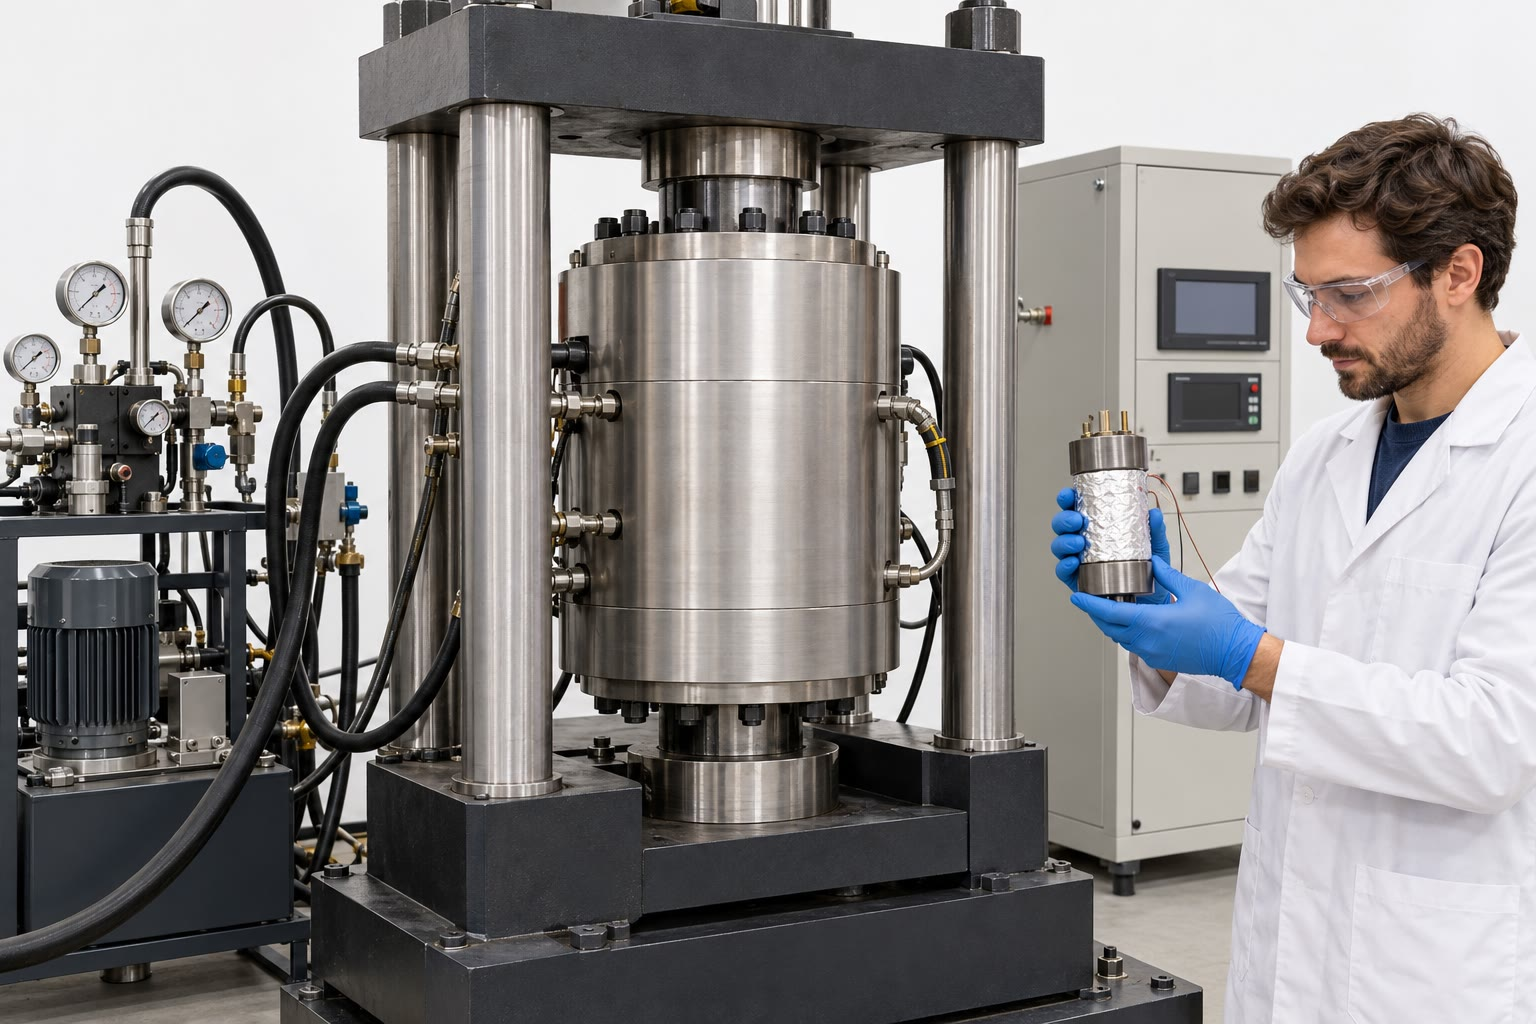
\includegraphics[width=\linewidth]{images/book5/ai/b3-deformation-press.jpg}

{\scriptsize 带套样品组装的岩石变形压机
（AI 生成示意图）。}

\smallskip
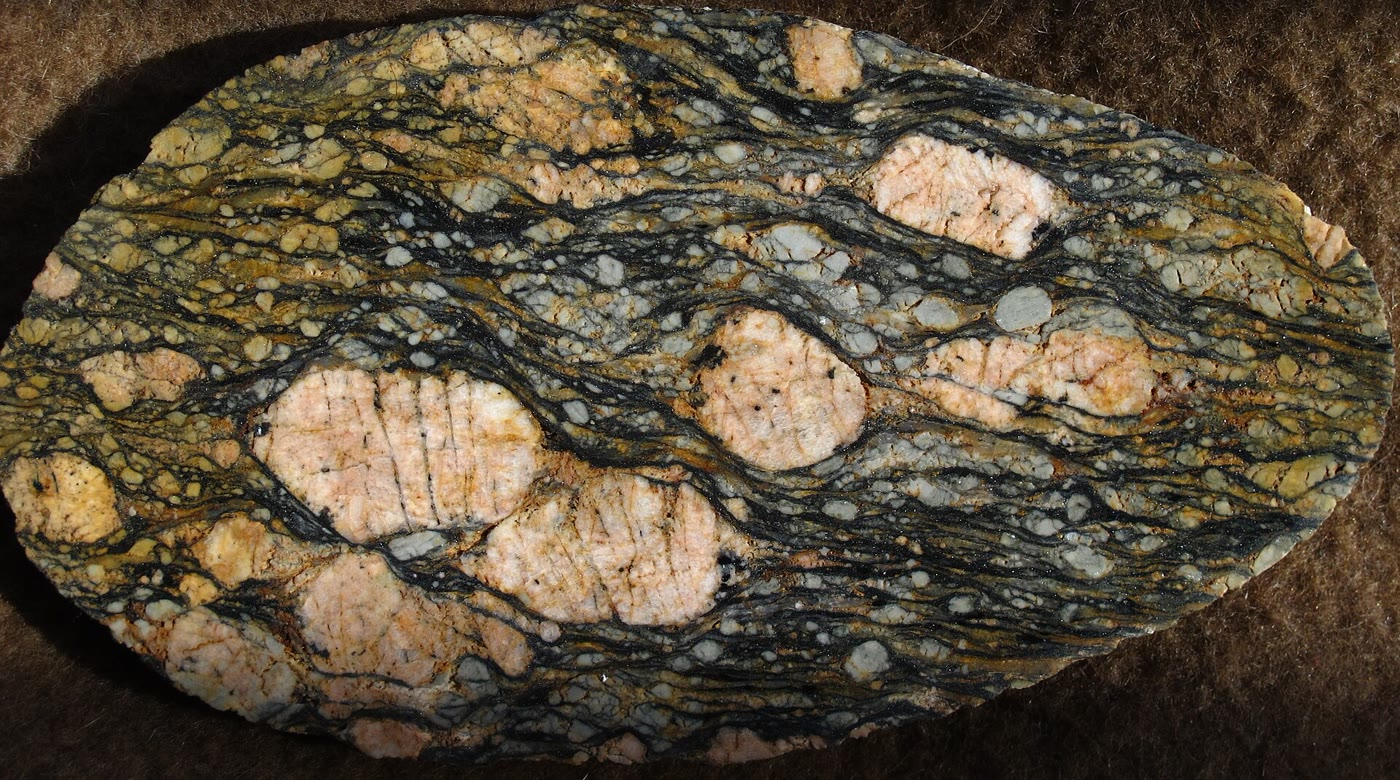
\includegraphics[width=\linewidth]{images/book5/b3-augen-mylonite.jpg}

{\scriptsize 取自挪威的锯切眼球状糜棱岩：大型长石残斑
位于由再结晶石英、长石和云母组成的细粒基质中。照片：
Mikenorton, CC BY-SA 4.0。}
\end{minipage}
\end{inthelab}
% ledger: mk00:diffusion, photo:b3-augen-mylonite

\section{练习}

\begin{exercise}[$\star$]\label{exo:b3:deformation-mechanisms:1}
镁橄榄石在 \qty{1890}{\celsius} 熔化，冰在 \qty{0}{\celsius} 熔化。计算
镁橄榄石在 \qty{1300}{\celsius} 时、冰在
\qty{-10}{\celsius} 时的\omterm{def:b3:deformation-mechanisms:flow-law}{同系温度}。哪一种更易蠕变？
\end{exercise}

\begin{exercise}[$\star$]\label{exo:b3:deformation-mechanisms:2}
一条与\omterm{def:b3:deformation-mechanisms:shear-zone}{剪切带}成直角穿过的岩墙，在带内被偏转了
\ang{70}，另一条偏转了 \ang{80}。计算剪应变。为什么大
应变难以这样测量？
\end{exercise}

\begin{exercise}[$\star$]\label{exo:b3:deformation-mechanisms:3}
用石英\omterm{def:b3:deformation-mechanisms:piezometer}{古应力计}，再结晶晶粒尺寸为
\qty{10}{\micro m} 时指示的应力是多少？
\end{exercise}

\begin{exercise}[$\star$]\label{exo:b3:deformation-mechanisms:4}
用湿石英岩的\omterm{def:b3:deformation-mechanisms:flow-law}{流动定律}（$A = \num{1.1e-4}$，$n = 4$，$E =
\qty{223}{kJ.mol^{-1}}$，$R = \qty{8.314}{J.mol^{-1}.K^{-1}}$），计算
在 \qty{500}{\celsius}、\qty{20}{MPa} 下的应变速率。
\end{exercise}

\begin{exercise}[$\star\star$]\label{exo:b3:deformation-mechanisms:5}
计算湿石英岩以 \qty{e-14}{s^{-1}} 的速率流动时的有效黏度，
分别在 \qty{400}{\celsius}（\qty{65.4}{MPa}）和 \qty{500}{\celsius}
（\qty{18.0}{MPa}）条件下的值。与
\cref{ch:b3:mantle-convection}中的\omterm{def:b3:mantle-convection:gia}{地幔黏度}作比较。
\end{exercise}

\begin{exercise}[$\star\star$]\label{exo:b3:deformation-mechanisms:6}
两次温度相同的实验得到 \qty{e-5}{s^{-1}}，
对应 \qty{100}{MPa}；另一次得到 \qty{1.6e-4}{s^{-1}}，
对应 \qty{200}{MPa}。计算\omterm{def:b3:deformation-mechanisms:flow-law}{应力指数}，并指出可能的机制。
\end{exercise}

\begin{exercise}[$\star\star$]\label{exo:b3:deformation-mechanisms:7}
在相同应力下，样品在 \qty{1100}{K} 时的蠕变速率
为 \qty{1000}{K} 时的十倍。计算活化能。
\end{exercise}

\begin{exercise}[$\star\star$]\label{exo:b3:deformation-mechanisms:8}
当晶粒尺寸除以十时，\omterm{def:b3:deformation-mechanisms:creep}{扩散蠕变}的应变速率
改变为原来的多少倍？分别对 纳巴罗–赫林蠕变和 科布尔蠕变回答。为什么
科布尔蠕变对晶粒尺寸更敏感？
\end{exercise}

\begin{exercise}[$\star\star$]\label{exo:b3:deformation-mechanisms:9}
对于 \qty{1100}{\celsius}、\qty{2}{GPa} 下的干橄榄石，两种\omterm{def:b3:deformation-mechanisms:flow-law}{流动定律}给出
$\dot\varepsilon_{\mathrm{dis}} = \num{6.54e-17}\,\sigma^{3.5}$ 和
$\dot\varepsilon_{\mathrm{dif}} = \num{3.59e-6}\,\sigma d^{-3}$（单位同正文）。
计算边界应力，分别对 $d = \qty{1}{mm}$ 和 $d =
\qty{100}{\micro m}$ 的情形，并求边界的斜率。
\end{exercise}

\begin{exercise}[$\star\star\star$]\label{exo:b3:deformation-mechanisms:10}
依据\cref{prop:b3:deformation-mechanisms:grain-size}的证明，
解释为什么晶格路径给出 $d^{-2}$，而边界路径给出 $d^{-3}$，并
证明边界扩散在晶粒尺寸 $d^* \approx
(B_B/B_L)\,\delta D_B/D_L$ 以下占主导。
\end{exercise}

\begin{exercise}[$\star\star\star$]\label{exo:b3:deformation-mechanisms:11}
对于 $n = 3.5$ 的\omterm{def:b3:deformation-mechanisms:flow-law}{流动定律}，应变速率增至原来的十倍时，
有效黏度降低为原来的多少倍？为什么这有利于应变
局部化形成\omterm{def:b3:deformation-mechanisms:shear-zone}{剪切带}？
\end{exercise}

\begin{exercise}[$\star\star\star$]\label{exo:b3:deformation-mechanisms:12}
在习题 9 的干橄榄石中，\qty{10}{MPa} 下的地幔\omterm{def:b3:deformation-mechanisms:shear-zone}{剪切带}
中的晶粒从 \qty{3}{mm} 再结晶为 \qty{30}{\micro m}。计算变化前后的总应变
速率，以及软化倍数。在每种情况下，
由哪种机制承担变形？
\end{exercise}

\section{问题：瓦尔登剪切带}

\begin{problem}[{周末问题——一条虚构剪切带的应变、应力、
应变速率与年龄}]
\label{pb:b3:deformation-mechanisms:1}
% values: calc/ch07.py; flow_laws.py; st03:piezometer, lopez:flow-laws
在瓦尔登丘陵花岗岩之下，即本系列虚构的区域内，
一个钻孔和一处深层公路路堑（二者均为虚构）揭示出一条韧性\omterm{def:b3:deformation-mechanisms:shear-zone}{剪切带}，
宽 \qty{400}{m}，形成于约 \qty{15}{km} 深度、\qty{450}{\celsius} 条件下。
一条与两壁成直角穿过的辉绿岩岩墙，在带内
与带的边界仅成 \ang{6} 的夹角。其中的石英是
由再结晶晶粒构成的糜棱岩，晶粒宽约 \qty{20}{\micro m}（从 15 到
\qty{25}{\micro m}）。取石英\omterm{def:b3:deformation-mechanisms:piezometer}{古应力计} $D = 10^{3.56}\sigma^{-1.26}$，
湿石英岩的\omterm{def:b3:deformation-mechanisms:flow-law}{流动定律}（$A = \num{1.1e-4}$，$n = 4$，$E =
\qty{223}{kJ.mol^{-1}}$），$R = \qty{8.314}{J.mol^{-1}.K^{-1}}$，\qty{1}{\text{年}} $=
\qty{3.156e7}{s}$，并在简单剪切中取 $\dot\gamma = 2\dot\varepsilon$。

\medskip\noindent\textbf{第一部分——应变。}
\begin{enumerate}
  \item 求岩墙的偏转角 $\psi$ 和剪应变。
  \item 求一壁相对于另一壁的位移。
  \item 求应变椭圆的主伸长比及其
        轴比。
  \item 求应变椭圆长轴与\omterm{def:b3:deformation-mechanisms:shear-zone}{剪切带}的夹角，
        并说明\omterm{def:b3:deformation-mechanisms:shear-zone}{剪切带}的面理随 $\gamma$ 增大如何变化？
  \item 俯视时，自南壁追踪该岩墙，它在进入东西向
        \omterm{def:b3:deformation-mechanisms:shear-zone}{剪切带}后向东弯折，到北壁处又恢复原来的
        向北方向。北壁向哪个方向移动？
        该\omterm{def:b3:deformation-mechanisms:shear-zone}{剪切带}是右行还是左行？
  \item 应沿哪个面切取薄片以读取\omterm{def:b3:deformation-mechanisms:kinematic}{运动学
        标志}，其 S 面理应如何倾斜？
\end{enumerate}

\medskip\noindent\textbf{第二部分——应力。}
\begin{enumerate}[resume]
  \item 求 \qty{20}{\micro m} 晶粒所指示的应力。
  \item 求晶粒为 15 和 \qty{25}{\micro m} 时的应力。
  \item 该应力是否在标定范围之内？
  \item \omterm{def:b3:deformation-mechanisms:piezometer}{古应力计}未显示出温度的影响，为何这一点
        在此处很重要？
  \item 应力为 \qty{100}{MPa} 时会产生多大的晶粒？
\end{enumerate}

\medskip\noindent\textbf{第三部分——应变速率。}
\begin{enumerate}[resume]
  \item 求 \qty{450}{\celsius} 时的 $E/RT$ 及阿伦尼乌斯因子。
  \item 求第 7 题所给应力下石英的应变速率
        （取 \qty{62}{MPa}）。
  \item 求剪应变速率。
  \item 求\omterm{def:b3:deformation-mechanisms:shear-zone}{剪切带}的有效黏度，并将其
        与\cref{ch:b3:mantle-convection}中的上地幔相比较。
  \item 在相同应力下，温度为 400 和
        \qty{500}{\celsius} 时，应变速率将分别改变多少倍？
  \item 若应力取最细晶粒所对应的 \qty{78}{MPa}，
        应变速率将改变多少倍？
\end{enumerate}

\medskip\noindent\textbf{第四部分——时间。}
\begin{enumerate}[resume]
  \item 求积累第 1 题中剪应变所需的时间，
        以秒计。
  \item 将其换算为千年。
  \item 求穿过\omterm{def:b3:deformation-mechanisms:shear-zone}{剪切带}的平均滑动速率，单位为 \unit{mm/\text{年}}。
  \item 将其与板块边界每年数十毫米的速率相比较。
        % ledger: morvel:range
  \item 若该\omterm{def:b3:deformation-mechanisms:shear-zone}{剪切带}以 \qty{20}{mm/\text{年}} 的速率滑动，其剪应变速率、应力
        以及再结晶晶粒尺寸各为多少？
  \item 晶粒尺寸和\omterm{def:b3:deformation-mechanisms:piezometer}{古应力计}指数的不确定度
        如何影响所求时间？
  \item 求瓦尔登\omterm{def:b3:deformation-mechanisms:shear-zone}{剪切带}积累其应变所用的时间，
        以千年计。
\end{enumerate}
\end{problem}
